\documentclass{xum_review}
%------------------------------------------------------------
% Packages
%------------------------------------------------------------
\usepackage{setspace}      % For line spacing
\usepackage{geometry}      % Page margins
\usepackage{fancyhdr}      % Header & footer
\usepackage{titlesec}      % Custom headings
\usepackage{csquotes}      % Quotation tools (optional)
\usepackage{listings}
\usepackage{xcolor} 
\usepackage{float}
\usepackage{caption}
% \usepackage{indentfirst}  % 注释掉以符合APA格式(首段不缩进)
\usepackage{graphicx}
\usepackage{amsmath}
\usepackage{adjustbox}
\usepackage{hyperref}
\usepackage{apacite}  % APA style with bibtex
\usepackage{tocloft}   % For customizing table of contents
\usepackage{hyperref}
\usepackage{cleveref}
\usepackage{lastpage}  % For getting total page count
\usepackage{fontspec}  % 添加fontspec包,XeLaTeX需要
% \usepackage{minted}  % 重新启用minted包


% XeLaTeX字体支持 - 添加Consolas字体
\setmonofont{Consolas}[Scale=0.9] % 设置等宽字体为Consolas,稍微缩放
% 或者如果想要更精细的控制:
% \newfontfamily\consolasfont{Consolas}[Scale=0.9]

% 代码格式 - 简约浅灰色风格,使用Consolas字体
\lstnewenvironment{python}[1][]
{
	% 添加语言标题 - 简约浅灰色窄条
	\vspace{0.5em}
	\noindent
	\colorbox[RGB]{232,232,232}{%
		\begin{minipage}{0.979\textwidth}
		\vspace{0.2em}
		\hspace{0.8em}
		
\includegraphics[height=0.9em]{figure/py_logo.png}%
		\hspace{0.5em}%
		\color[RGB]{88,88,88}%
		\textbf{\textsf{Python}}%
		\vspace{0.2em}
		\end{minipage}
	}
	\vspace{-1.65em}
	\lstset{
		language=Python,
		basicstyle=\ttfamily\footnotesize, % XeLaTeX会自动使用Consolas
		numbers=left,
		numberstyle=\ttfamily\color[RGB]{130,130,130},
		numbersep=5pt,
		frame=none,
		framesep=0pt,
		xleftmargin=0pt,
		framexleftmargin=0pt,
		% backgroundcolor=\color[RGB]{255,255,255},
		backgroundcolor=\color[RGB]{245,245,245},
		breaklines=true,
		breakindent=10pt,
		keywordstyle=\color[RGB]{255,119,0},
		morekeywords={as, self},
		deletekeywords={print},
		keywordstyle=[2]\color[RGB]{144,0,144},
		morekeywords=[2]{print},
		stringstyle=\color[RGB]{0,170,0},
		commentstyle=\color[RGB]{221,0,0},
		showstringspaces=false,
		#1
	}
}{}

%JSON代码格式 - 简约浅灰色风格
\lstnewenvironment{json}[1][]
{
	% 添加JSON语言标题 - 简约浅灰色窄条
	\vspace{0.5em}
	\noindent
	\colorbox[RGB]{232,232,232}{%
		\begin{minipage}{0.979\textwidth}
		\vspace{0.2em}
		\hspace{0.8em}
		
\includegraphics[height=0.9em]{figure/json_logo.png}%
		\hspace{0.5em}%
		\color[RGB]{88,88,88}%
		\textbf{\textsf{JSON}}%
		\vspace{0.2em}
		\end{minipage}
	}
	\vspace{-1.65em}
	\lstset{
		language=,
		basicstyle=\ttfamily\footnotesize,
		numbers=left,
		numberstyle=\ttfamily\color[RGB]{130,130,130},
		numbersep=5pt,
		frame=none,
		framesep=0pt,
		xleftmargin=0pt,
		framexleftmargin=0pt,
		% framexleftmargin=2pt,
		% backgroundcolor=\color[RGB]{255,255,255},
		backgroundcolor=\color[RGB]{245,245,245},
		breaklines=true,
		breakindent=10pt,
		% JSON特有的语法高亮
		stringstyle=\color[RGB]{0,170,0},      % 字符串为绿色
		keywordstyle=\color[RGB]{0,0,255},     % 关键字为蓝色
		% numberstyle=\color[RGB]{255,119,0},    % 数字为橙色
		commentstyle=\color[RGB]{221,0,0},     % 注释为红色(虽然JSON标准不支持注释)
		% 定义JSON的特殊字符高亮
		literate=
		{:}{{{\color[RGB]{255,119,0}{:}}}}{1}
		{,}{{{\color[RGB]{255,119,0}{,}}}}{1}
		{\{}{{{\color[RGB]{0,0,255}{\{}}}}{1}
		{\}}{{{\color[RGB]{0,0,255}{\}}}}}{1}
		{[}{{{\color[RGB]{0,0,255}{[}}}}{1}
		{]}{{{\color[RGB]{0,0,255}{]}}}}{1}
		{true}{{{\color[RGB]{144,0,144}{true}}}}{4}
		{false}{{{\color[RGB]{144,0,144}{false}}}}{5}
		{null}{{{\color[RGB]{144,0,144}{null}}}}{4},
		showstringspaces=false,
		morestring=[b]",
		morestring=[b]',
		#1
	}
}{}

\lstnewenvironment{cmd}[1][]
{
	% 添加 Windows CMD 语言标题 - 仿CMD窗口深色风格
	\vspace{0.5em}
	\noindent
	\colorbox[RGB]{232,232,232}{%
	\begin{minipage}{0.914\textwidth}
		\vspace{0.2em}
		\hspace{0.8em}
		% 这里可以放一个CMD的图标,如果没有可以注释掉
		
\includegraphics[height=0.9em]{figure/WIndows-Terminal-icon.png}%
		\hspace{0.5em}%
		\color[RGB]{88,88,88}%
		\textbf{\textsf{Windows Command Prompt}}%
		\vspace{0.2em}
		\end{minipage}
	}
	\vspace{-2em}
	\lstset{
		language=command.com, % 设置语言为 command.com (适用于DOS/CMD)
		basicstyle=\ttfamily\footnotesize, % 浅色文字
		numbers=left,
		numberstyle=\ttfamily\color[RGB]{170,170,170}, % 数字颜色
		numbersep=5pt,
		frame=none,
		framesep=0pt,
		xleftmargin=0pt,
		framexleftmargin=0pt,
		backgroundcolor=\color[RGB]{245,245,245}, % 深色背景
		breaklines=true,
		breakindent=10pt,
		% CMD/Batch 语法高亮
		stringstyle=\color[RGB]{255,255,0},      % 字符串为黄色
		keywordstyle=\color[RGB]{0,255,255},     % 关键字为青色
		commentstyle=\color[RGB]{0,170,0},     % 注释 (REM) 为绿色
		showstringspaces=false,
		morestring=[b]",
		morestring=[b]',
		#1
	}
}{}

%HTML代码格式 - 简约浅灰色风格
\lstnewenvironment{html}[1][]
{
	% 添加HTML语言标题 - 简约浅灰色窄条
	\vspace{0.5em}
	\noindent
	\colorbox[RGB]{232,232,232}{%
		\begin{minipage}{0.979\textwidth}
		\vspace{0.2em}
		\hspace{0.8em}%
		
\includegraphics[height=1em]{figure/html_logo.png}%
		\hspace{0.5em}%
		\color[RGB]{88,88,88}%
		\textbf{\textsf{HTML}}%
		\vspace{0.2em}
		\end{minipage}
	}
	\vspace{-1.65em}
	\lstset{
		language=HTML,
		basicstyle=\ttfamily\footnotesize,
		numbers=left,
		numberstyle=\ttfamily\color[RGB]{130,130,130},
		numbersep=5pt,
		frame=none,
		framesep=0pt,
		xleftmargin=0pt,
		framexleftmargin=0pt,
		backgroundcolor=\color[RGB]{245,245,245},
		breaklines=true,
		breakindent=10pt,
		% HTML特有的语法高亮
		keywordstyle=\color[RGB]{0,0,255},        % HTML标签为蓝色
		stringstyle=\color[RGB]{0,170,0},         % 字符串为绿色
		commentstyle=\color[RGB]{221,0,0},        % 注释为红色
		identifierstyle=\color[RGB]{255,119,0},   % 属性为橙色
		showstringspaces=false,
		tabsize=2,
		#1
	}
}{}

%JavaScript代码格式 - 简约浅灰色风格
\lstnewenvironment{javascript}[1][]
{
	% 添加JavaScript语言标题 - 简约浅灰色窄条
	\vspace{0.5em}
	\noindent
	\colorbox[RGB]{232,232,232}{%
		\begin{minipage}{0.979\textwidth}
		\vspace{0.2em}
		\hspace{0.8em}
		
\includegraphics[height=1em]{figure/js_logo.png}%
		\hspace{0.5em}%
		\color[RGB]{88,88,88}%
		\textbf{\textsf{JavaScript}}%
		\vspace{0.2em}
		\end{minipage}
	}
	\vspace{-1.65em}
	\lstset{
		language=Java,
		basicstyle=\ttfamily\footnotesize,
		numbers=left,
		numberstyle=\ttfamily\color[RGB]{130,130,130},
		numbersep=5pt,
		frame=none,
		framesep=0pt,
		xleftmargin=0pt,
		framexleftmargin=0pt,
		backgroundcolor=\color[RGB]{245,245,245},
		breaklines=true,
		breakindent=10pt,
		% JavaScript特有的语法高亮
		keywordstyle=\color[RGB]{144,0,144},      % 关键字为紫色
		keywordstyle=[2]\color[RGB]{255,119,0},   % 函数名为橙色
		morekeywords={var,let,const,function,return,if,else,for,while,do,switch,case,break,continue,try,catch,finally,throw,new,this,typeof,instanceof,in,of,async,await,class,extends,super,static,import,export,default,from,as},
		morekeywords=[2]{console,document,window,alert,prompt,confirm,getElementById,createElement,appendChild,addEventListener,fetch,Promise,JSON,Array,Object,String,Number,Boolean,Date,RegExp,Math,parseInt,parseFloat,isNaN,setTimeout,setInterval,clearTimeout,clearInterval},
		stringstyle=\color[RGB]{0,170,0},         % 字符串为绿色
		commentstyle=\color[RGB]{221,0,0},        % 注释为红色
		identifierstyle=\color[RGB]{0,0,0},       % 标识符为黑色
		showstringspaces=false,
		tabsize=2,
		morecomment=[l]{//},
		morecomment=[s]{/*}{*/},
		morestring=[b]",
		morestring=[b]',
		morestring=[b]`,
		#1
	}
}{}

% 通用代码环境 - 简约浅灰色风格
\newcommand{\codeheader}[1]{%
	\vspace{0.5em}
	\noindent
	\colorbox[RGB]{248,249,250}{%
		\begin{minipage}{\textwidth}
		\vspace{0.2em}
		\hspace{0.8em}
		\color[RGB]{88,88,88}%
		\textbf{\textsf{#1}}%
		\vspace{0.2em}
		\end{minipage}
	}
	\vspace{-0.1em}
}

\lstnewenvironment{codewithheader}[2][]
{
	\codeheader{#2}
	\lstset{
		basicstyle=\ttfamily\footnotesize,
		numbers=left,
		numberstyle=\tiny\color{gray},
		numbersep=8pt,
		frame=single,
		framerule=0.5pt,
		frameround=ffff,
		rulecolor=\color[RGB]{229,230,232},
		framesep=2pt,
		xleftmargin=0pt,
		framexleftmargin=2pt,
		backgroundcolor=\color[RGB]{255,255,255},
		breaklines=true,
		breakindent=10pt,
		keywordstyle=\color[RGB]{255,119,0},
		stringstyle=\color[RGB]{0,170,0},
		commentstyle=\color[RGB]{221,0,0},
		showstringspaces=false,
		#1
	}
}{}

% ===============================================
% VS Code 风格的 minted 环境(需要 --shell-escape)
% ===============================================

% 设置全局minted样式
% \usemintedstyle{monokai}

% % VS Code 风格的 Python 环境
% \newenvironment{vscode-python}[1][]
% {%
% 	% VS Code风格的深色标题栏
% 	\vspace{0.5em}%
% 	\noindent
% 	\colorbox[RGB]{30,30,30}{%
% 		\begin{minipage}{\textwidth}
% 		\vspace{0.2em}
% 		\hspace{0.8em}
% 		
\includegraphics[height=0.9em]{figure/py_logo.png}%
% 		\hspace{0.5em}%
% 		\color[RGB]{204,204,204}%
% 		\textbf{\textsf{Python}}%
% 		\vspace{0.2em}
% 		\end{minipage}
% 	}%
% 	\vspace{-0.1em}%
% 	\begin{minted}[
% 		style=monokai,
% 		bgcolor=black,
% 		fontsize=\footnotesize,
% 		linenos,
% 		numbersep=8pt,
% 		xleftmargin=10pt,
% 		framesep=2mm,
% 		#1
% 	]{python}%
% }{%
% 	\end{minted}%
% }

% % VS Code 风格的 JSON 环境
% \newenvironment{vscode-json}[1][]
% {%
% 	% VS Code风格的深色标题栏
% 	\vspace{0.5em}%
% 	\noindent
% 	\colorbox[RGB]{30,30,30}{%
% 		\begin{minipage}{\textwidth}
% 		\vspace{0.2em}
% 		\hspace{0.8em}
% 		
\includegraphics[height=0.9em]{figure/json_logo.png}%
% 		\hspace{0.5em}%
% 		\color[RGB]{204,204,204}%
% 		\textbf{\textsf{JSON}}%
% 		\vspace{0.2em}
% 		\end{minipage}
% 	}%
% 	\vspace{-0.1em}%
% 	\begin{minted}[
% 		style=monokai,
% 		bgcolor=black,
% 		fontsize=\footnotesize,
% 		linenos,
% 		numbersep=8pt,
% 		xleftmargin=10pt,
% 		framesep=2mm,
% 		#1
% 	]{json}%
% }{%
% 	\end{minted}%
% }



\lstnewenvironment{htmlcssjs}[1][]
{
	% 添加HTML CSS JavaScript语言标题 - 简约浅灰色窄条
	\vspace{0.5em}
	\noindent
	\colorbox[RGB]{232,232,232}{%
		\begin{minipage}{0.979\textwidth}
		\vspace{0.2em}
		\hspace{0.8em}
		\includegraphics[height=0.9em]{figure/html_css_js_logo.png}%
		\hspace{0.5em}%
		\color[RGB]{88,88,88}%
		\textbf{\textsf{HTML CSS JavaScript}}%
		\vspace{0.2em}
		\end{minipage}
	}
	\vspace{-1.65em}
	\lstset{
		language=HTML,
		basicstyle=\ttfamily\footnotesize,
		numbers=left,
		numberstyle=\ttfamily\color[RGB]{130,130,130},
		numbersep=5pt,
		frame=none,
		framesep=0pt,
		xleftmargin=0pt,
		framexleftmargin=0pt,
		backgroundcolor=\color[RGB]{245,245,245},
		breaklines=true,
		breakindent=10pt,
		% HTML CSS JavaScript特有的语法高亮
		keywordstyle=\color[RGB]{0,0,255},        % HTML标签为蓝色
		stringstyle=\color[RGB]{0,170,0},         % 字符串为绿色
		commentstyle=\color[RGB]{221,0,0},        % 注释为红色
		identifierstyle=\color[RGB]{255,119,0},   % 属性为橙色
		showstringspaces=false,
		tabsize=2,
		#1
	}
}{}

\begin{document}

\tableofcontents
\newpage
\setcounter{page}{1}

\section{Introduction}

Intelligent Q\&A systems have seen growing use in education, customer service,
and online consultation. With advances in NLP, machine learning, and large
language models (LLMs), chatbots are now more capable of understanding complex
queries and managing multi-turn conversations.

In university settings, students often face practical questions related to
course schedules, administrative procedures, and campus facilities. Traditional
methods of information access such as browsing websites or asking peers can be
time-consuming and inefficient. 

This project aims to design and implement a chatbot tailored to student inquiry
scenarios. It accurately detects user intent, recognizes key entities, and
generates responses based on a built-in campus information knowledge base. By
integrating multiple NLU components, including intent classification, entity
recognition, and sentiment analysis, the system enhances user experience and
improves overall information availability on campus.

\section{Project Methodology}

	\subsection{Research Design and Paradigm}

	This project adopts the Constructive Research / Design Science (DSR)
	research paradigm. The core objective is to design, build, and evaluate a
	novel intelligent system—a hybrid chatbot that integrates both
	retrieval-based and template-based features—to address real-world problems
	such as low information retrieval efficiency and lack of emotional
	interaction in campus
	settings\citep{yang2019hybridretrievalgenerationneuralconversation}.

	\noindent The overall research process follows an iterative development cycle:
	\begin{enumerate}
		\item	Requirement Analysis and Data Collection: Identify key
		information needs in campus scenarios and gather relevant raw data.
		\item	System Design and Implementation: Design and build a system
		architecture comprising a Natural Language Understanding (NLU) module, a
		response generation module, and an interactive front-end interface.
		\item	Model Training and Development: Train the core NLU model using
		synthetic data generated by LLM and inspected by human.
		\item	System Integration and Evaluation: Integrate all modules into a
		working prototype and evaluate the system using both quantitative and
		qualitative methods.
		\item	Iterative Optimization: Refine the system by enriching training
		data and optimizing components based on evaluation feedback.
	\end{enumerate}

	This design-oriented research approach ensures that the outcomes are not
	only theoretically grounded but also practically valuable. The iterative
	methodology further enables rapid feedback incorporation and continuous
	system improvement in real-world usage scenarios.

	\subsection{System Architecture}

	The chatbot system follows a reasonable architecture as
	\citet{mohammed2022chatbotarchitecture} adopted in their research,
	consisting of a frontend user interface and a backend processing core. The
	backend adopts a modular design, primarily comprising a Natural Language
	Understanding (NLU) module and a response generation module. The overall
	architecture is shown in \cref{fig:system_architecture}. The functions
	of each component will be described in detail in the following subsection.


	%d figure needs modify
	\begin{figure}[H]
		\centering
		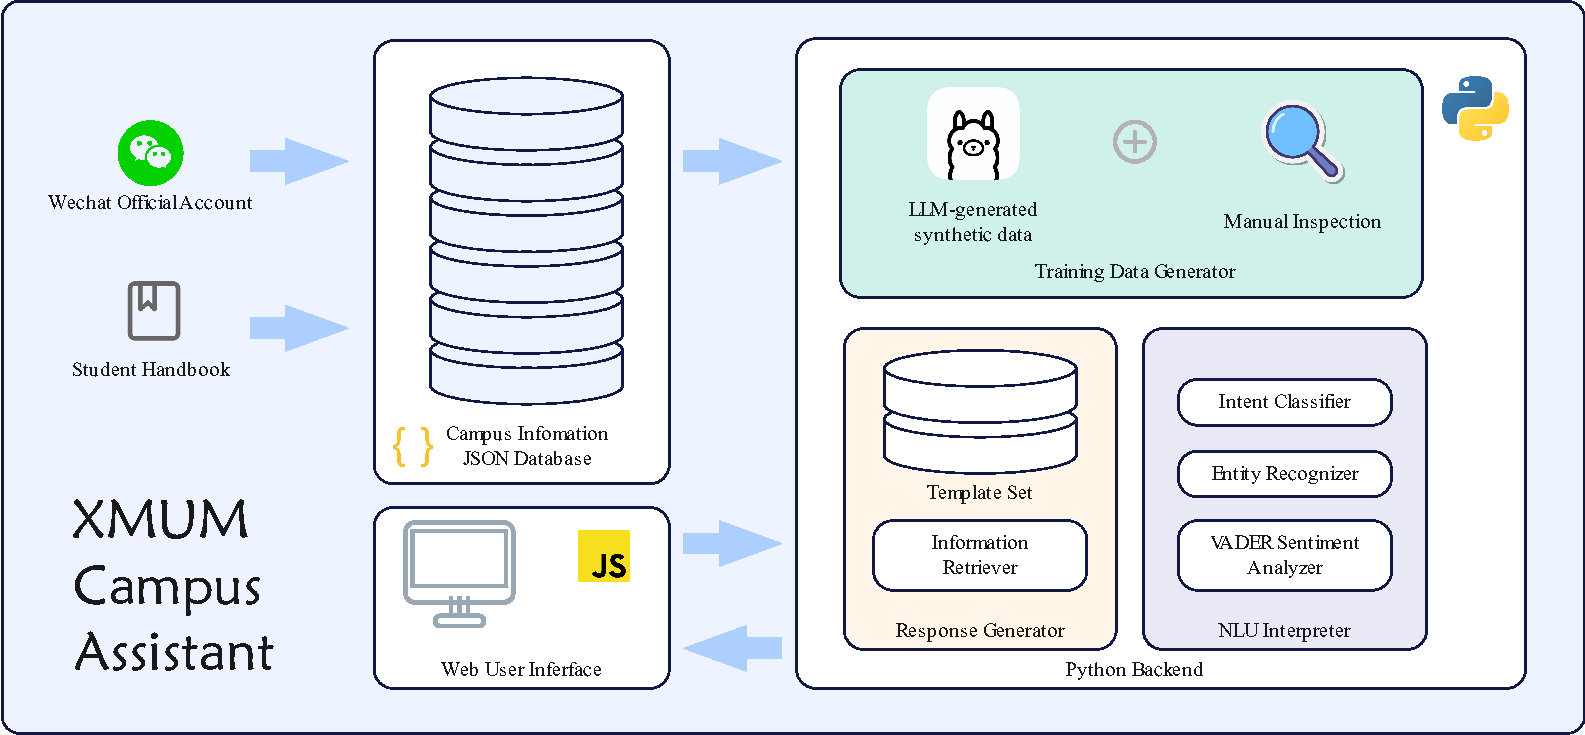
\includegraphics[width=1\textwidth]{figure/overall_flowchart.pdf}
		\caption{Overall System Architecture}
		\label{fig:system_architecture}
	\end{figure}


	\subsection{Data Collection and Preparation}

	High-quality data is fundamental to the performance of natural language
	processing systems. In this study, data collection was conducted on two
	levels: (1) organizing raw information for knowledge base construction, and
	(2) generating training corpora for the NLU model. Both types of data
	underwent structured processing and manual verification to ensure their
	usability and reliability in system development.

	\subsubsection{Knowledge Base Data}
	We manually collected information on campus facilities, dining options,
	academic procedures, and more by consulting the student handbook, official
	public accounts, and other campus information sources, and structured it
	into a searchable \texttt{JSON} file as the knowledge base of the intelligent
	system. Here is a snippet of the knowledge base:

	\begin{json}
"restaurant": {
	"possible_intent": ["ask_restaurant_location", "ask_restaurant_time", "ask_restaurant_recommendation"],
	"starbucks": {
		"restaurant_name": "Starbucks",
		"possible_name": ["Starbucks", "starbucks", "STARBUCKS"],
		"location": "Bell Avenue Roadside",
		"opening_hours": "9:00-21:00",
		"recommendation_reason": "It's a coffee shop with various drinks and snacks"
	},
	...
}
	\end{json}


	\subsubsection{Model Training Data}
	
	Since we will adopt supervised learning to train the NLU model (which will
	be introduced in \cref{sec:nlu}), a large amount of training data is needed.
	However, preparing them completely manually will be extremely
	time-consuming. Thus, we adopted a \textit{synthetic data} strategy.
	Specifically, we first designed a data generator
	(\texttt{data\_generator.ipynb}) that fills predefined intents and entities
	into prompt templates. Then, a locally deployed \texttt{Ollama} LLM is used
	to generate many feature-label pairs. Finally, all generated data must
	undergo \textbf{manual sampling, review, and correction} to ensure quality
	and accuracy before being used for model training as
	\citet{li2024datagenerationusinglarge} stressed in their research.

	\subsection{Evaluation Methods}

	To comprehensively evaluate the effectiveness of this project, we adopted a
	combination of quantitative and qualitative assessment
	methods\citep{0b014ee667a84c5985984bfd771595a3}.

	\subsubsection{Quantitative Evaluation}
	
	The evaluation primarily focuses on the performance of the NLU model. We
	used an independent test set and employed scikit-learn's
	\texttt{classification\_report} tool to automatically calculate a range of
	model evaluation metrics, including precision, recall, and F1-score—derived
	from the confusion matrix—to assess the model's performance across each
	class\citep{scikit-learn_classification_report_nd}.

	\subsubsection{Qualitative Evaluation}

	The evaluation primarily targets the overall user experience and
	practicality of the chatbot system. We conducted multi-turn, open-ended
	conversations with the chatbot, with a particular focus on its ability to
	handle edge cases beyond the training data. This allowed us to assess the
	fluency of the dialogue, the accuracy of the responses, and the
	effectiveness of emotional interaction.

\section{Design of the Intelligent System}

	\subsection{Core Modules and Their Functions}

	\subsubsection{User Input Interface}

	This module is responsible for capturing user input and sending it to the
	back-end interpretation module. We adopted a Web UI architecture, with the
	frontend built using \texttt{JavaScript} and \texttt{HTML}, and connected to
	the Python backend via the \texttt{Flask} framework.

	\subsubsection{Natural Language Understanding (NLU) Module}\label{sec:nlu}

	The Natural Language Understanding (NLU) module serves as the system's
	initial processing stage, responsible for transforming users' free-form text
	input into structured semantic information\citep{article}. It consists of
	the following three subsystems:

	\begin{itemize}
		\item{\textbf{Intent Classification}}\\
		This model aims to identify the user's query intent within a specific
		context. The task is formulated as a multi-class text classification
		problem, which we adopt supervised learning to solve it:
		\begin{enumerate}
			\item Prepare labeled data for model training and use split it into
			train set and test set.

			\item Construct a Scikit-learn \texttt{Pipeline} consisting \textit{TF-IDF
			vectorizer} and \textit{logistic regression} and train the model\citep{batra-2023}.
			
			\item Check the \texttt{classification\_report} and generate more training data to improve the performance 
			of the intent classifier.\\
			For example, we once get the classification report below:
	\begin{table}[H] 
		\centering
		\caption{Classification Report of Intent Classifier (sorted by number of training data)}
		\label{tab:classification_report} 
		
		\begin{tabular}{l c c c c c} 
		\hline % 表格顶部粗线
		\textbf{Category} & \textbf{Precision} & \textbf{Recall} & \textbf{F1-score} & \textbf{Support} & \textbf{Training Data} \\
		\hline % 表格中部细线
		ask\_handbook\_info & 0.965 & 0.991 & 0.978 & 110 & 482 \\
		ask\_restaurant\_time & 0.982 & 0.991 & 0.987 & 112 & 452 \\
		ask\_restaurant\_location & 0.949 & 0.970 & 0.960 & 135 & 419 \\
		ask\_facility\_time & 0.812 & 0.897 & 0.852 & 29 & 155 \\
		ask\_facility\_info & 0.857 & 0.667 & 0.750 & 36 & 139 \\
		ask\_facility\_location & 0.730 & 0.794 & 0.761 & 34 & 123 \\
		ask\_building\_location & 0.786 & 0.647 & 0.710 & 17 & 67 \\
		greet\_welcome & 0.385 & 0.625 & 0.476 & 8 & 58 \\
		greet\_sorry & 1.000 & 0.917 & 0.957 & 12 & 56 \\
		ask\_building\_include & 1.000 & 0.667 & 0.800 & 12 & 50 \\
		greet\_hello & 0.455 & 0.385 & 0.417 & 13 & 45 \\
		greet\_thanks & 1.000 & 1.000 & 1.000 & 11 & 41 \\
		greet\_goodbye & 0.800 & 0.364 & 0.500 & 11 & 39 \\
		\hline % 汇总数据前的细线
		\textbf{Accuracy} & \multicolumn{3}{c}{0.910} & 641 & \\ 
		\textbf{Macro Avg} & 0.833 & 0.779 & 0.793 & 641 & \\
		\textbf{Weighted Avg} & 0.911 & 0.910 & 0.907 & 641 & \\
		\hline % 表格底部粗线
		\end{tabular}
	\end{table}
		We can observe from \cref{tab:classification_report} that the more
		training data we have, the better the performance of the intent
		classifier is. Also, it's worth noting that some categories, such as
		\texttt{greet\_thanks} seem to have a very high precision score but have low
		amount of training data. This may be attributed to the limited size of
		the test dataset, potentially leading to \textbf{sampling bias} or
		\textbf{overfitting}.

		Eventually, we obtain more synthetic data for those categories with small amount
		of training data and enhance the overall performance of the intent classifier.

		\end{enumerate}
		
		
		
		\item{\textbf{Entity Recognition}}\\
		To further extract key information from user input (such as location,
		time, or objects), we need to recognize entities. This task is modeled as 
		Named Entity Recognition (NER) in sequence labeling problem\citep{singh-2024}. We adopt the 
		following procedures to solve it:
		\begin{enumerate}
			\item Prepare labeled data for model training and convert it to the tuple data format required by \texttt{spaCy}. 
			Example:\\
			\texttt{[('Where is Xia Yi Cheng located?', {'entities': [(9, 21, 'restaurant')]})]}
			\item Train a \texttt{spaCy} model to recognize it.
			\item Check the model performance using a self-built classification report and increase training data amount
			accordingly.
		\end{enumerate}
		
		\item{\textbf{Sentiment Analysis}}\\
		To enhance the system's human-centered and emotional awareness
		capabilities, the \textit{VADER sentiment analysis} tool is integrated
		to classify the emotional tone and intensity of user input\citep{Hutto_Gilbert_2014}. The output
		includes positive, negative, and neutral sentiment categories, along
		with a compound score, which informs template selection and interaction
		tone adjustment.
	\end{itemize}

	\subsubsection{Response Generation Module}

	The response generation module is responsible for producing
	user-understandable and naturally styled text replies based on the intent,
	entities, and sentiment data output by the NLU module. It comprises the
	following two core components:

	\begin{itemize}
		\item{\textbf{Knowledge Base Retriever}}\\
		The system's knowledge is organized in a structured JSON format,
		covering common campus inquiry scenarios. The retriever receives
		keywords and labels from the NLU module and performs matching queries
		within the knowledge base to locate the most relevant information
		entries.
		\item{\textbf{Response Templating Engine}}\\
		A hierarchical response templating strategy is employed, with
		standardized language templates designed for different intent types and
		sentiment labels.Based on the user's identified intent, extracted
		entities, and sentiment scores, the engine dynamically selects the
		appropriate template and fills in placeholders with information
		retrieved from the knowledge base, ultimately generating coherent and
		complete natural language responses.
	\end{itemize}

	\subsubsection{Interactive Front-end Interface}

	The front-end interface is built using a web framework and provides a
	chat-like, turn-based interaction experience.

	\subsection{Data Flow and Workflow}

	The system operates based on a single-turn interaction model following the
	sequence: \textit{Input → Interpretation → Generation → Output}. For each
	user query, the system sequentially invokes its modules and returns a
	structured, readable response. The following describes a typical data flow
	during system operation.

	%d insert figure

	\subsubsection{Input Stage}

	System operation begins when the user submits a natural language query
	through the input interface, such as "Where is Starbucks located?".
	Before entering the main processing pipeline, the input is first passed
	through a sentence segmentation step to enable sentence-by-sentence analysis
	for multi-sentence queries.

	\subsubsection{Natural Language Understanding Stage}

	Once the input text enters the Natural Language Understanding (NLU) module,
	it undergoes the following processing steps in sequence:
	\begin{itemize}
		\item	The intent classifier detect the intent of user input, such as
	 \texttt{ask\_facility\_location} or \texttt{ask\_restaurant\_time}.
		\item	The entity recognizer extracts key entities from the input, such
		as \texttt{Starbucks: restaurant} or \texttt{library: facility}, to
		support content generation in the response module.
		\item	The VADER sentiment analyzer detect the sentiment score of user input
		and categorize it into three tags: positive, neutral, and negative.
	\end{itemize}

	After each clause is processed, the system organizes the output into a
	unified intermediate format. For example, given the input "Where is
	Starbucks located?", the structured output is:

	\begin{json}
	{ 
		"query": "Where is Starbucks located?",
		"intent": "ask_restaurant_loaction",
		"entities": {"Starbucks": "restaurant"}
		"sentiment_tag": "neutral"
	}
	\end{json}

	The whole NLU process is shown in \cref{fig:nlu_process}.

	\begin{figure}[H]
		\centering
		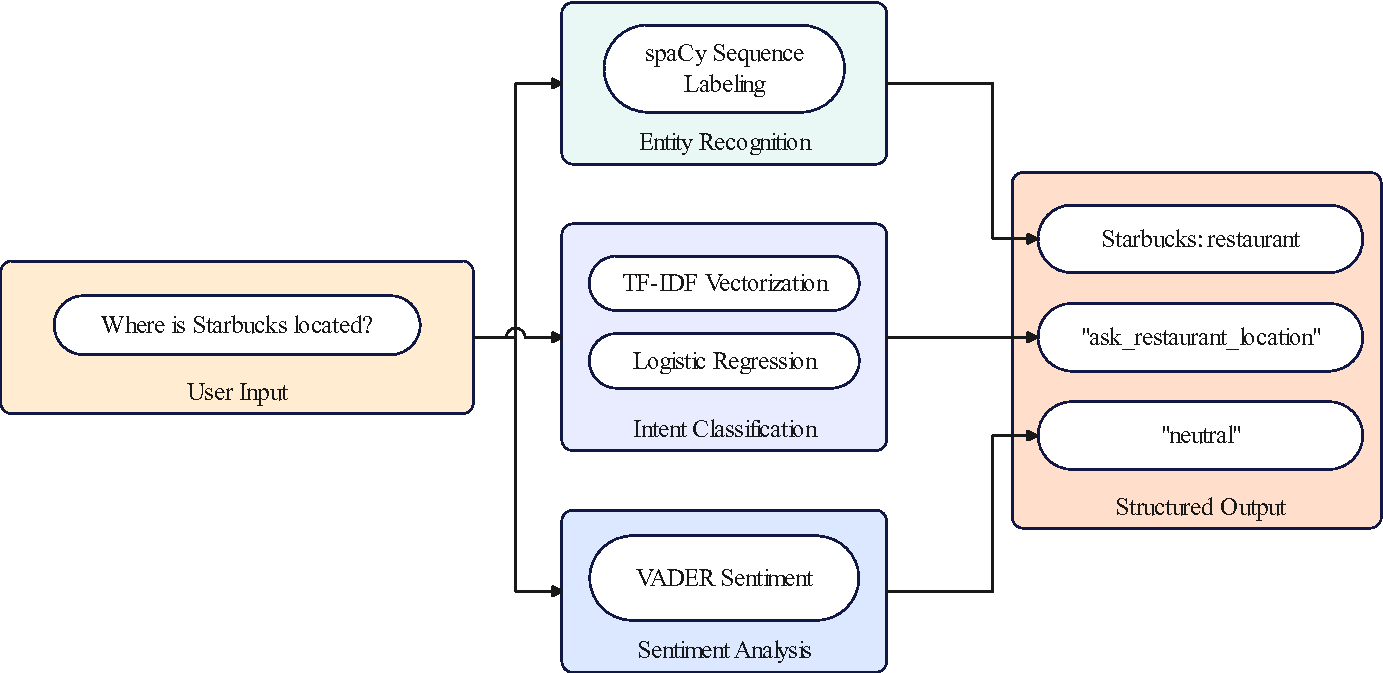
\includegraphics[width=1\textwidth]{figure/nlu_flow.pdf}
		\caption{NLU Process Flow Chart}
		\label{fig:nlu_process}
	\end{figure}

	\subsubsection{Response Generation Stage}

	Based on the structured output, the system invokes the response generation
	module. It will first match the correct output template according to
	the intent and sentiment and retrieve in the knowledge base for information
	to be filled in the template.

	For instance, if the module receive the output above, it will find the following
	template:\\
	\begin{json}
	{
	"ask_restaurant_location":{
		"info":["restaurant_name","location"],
		"neutral": "{restaurant_name} can be found at {location}.",
	}
	}
	\end{json}

	And it will retrieve in the knowledge base for \texttt{restaurant\_name} and \texttt{location}
	of Starbucks until it finds:\\
	\begin{json}
	"starbucks": {
      "restaurant_name": "Starbucks",
      "possible_name": ["Starbucks", "starbucks", "STARBUCKS"],
      "location": "Bell Avenue Roadside",
      "opening_hours": "9:00-21:00",
      "recommendation_reason": "It's a coffee shop with various drinks and snacks"
    }
	\end{json}

	The whole response generation process is shown in \cref{fig:response_generation_process}.

	\begin{figure}[H]
		\centering
		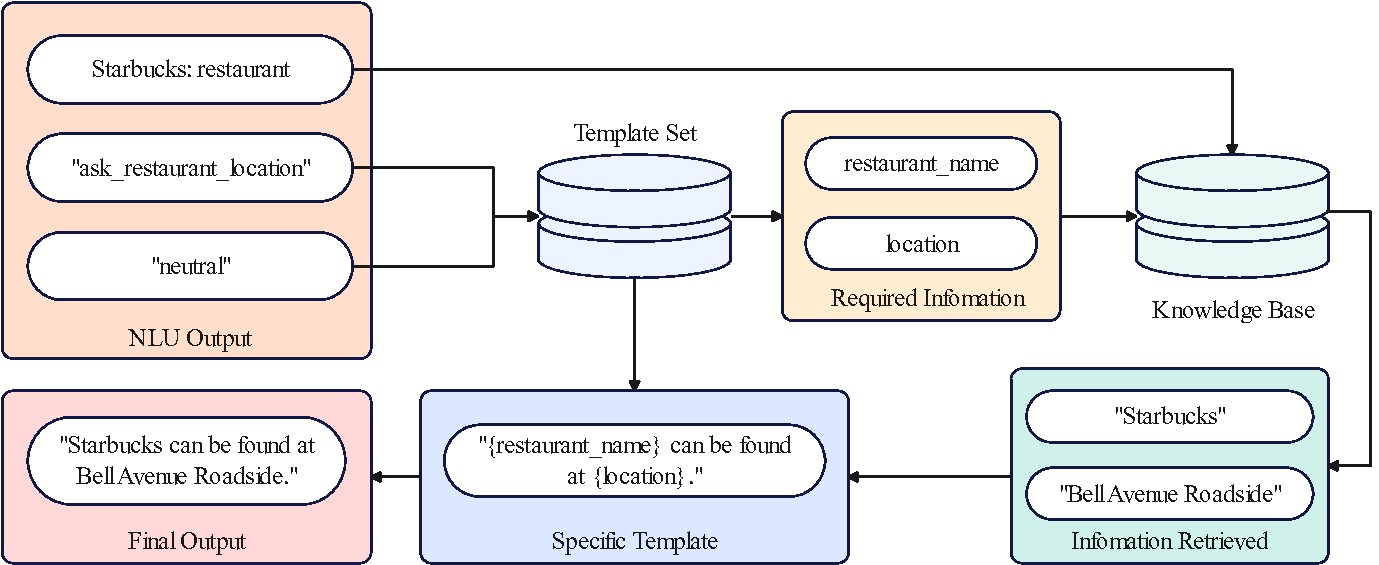
\includegraphics[width=1\textwidth]{figure/response.pdf}
		\caption{Response Generation Process Flow Chart}
		\label{fig:response_generation_process}
	\end{figure}

	\subsubsection{Output Stage}

	The final response will be transmitted from the Python backend to the Web UI
	for display, using the \texttt{Flask} framework.

\section{Implementation}
    
	Before the implementation, kindly refer to \cref{sec:appendix} for the runtime dependencies
	of this intelligent system.
	

	% \subsection{System Architecture and Modules}

	% \subsection{Prototype Screenshots}

	% \subsection{System Execution and Testing}

\section{Discussion}

	\subsection{Summary of Overall Effectiveness}

	This system is designed to improve information access for XMUM
	students and enhance the accessibility of campus-related content. During
	development, a modular architecture was adopted to facilitate system
	construction and deployment.

	Evaluation results indicate that the system performs reliably in intent
	classification and entity recognition, effectively covering most common
	campus-related queries. The sentiment analysis module also contributed to
	tone adjustment in responses, enhancing the naturalness and
	user-friendliness of interactions. Although the current version does not yet
	support multi-turn dialogue or context modeling, it has demonstrated task
	completion and user experience in single-turn scenarios, meeting the
	intended design goals.


	\subsection{Advantages of Models and Systems}

	%e subject to change
	The system demonstrates several key strengths in both core modeling and
	overall architectural design. Firstly, the NLU module performed well on the
	test set, showing high accuracy and stability, which provides a reliable
	foundation for information retrieval. The response generator can match
	template and retrieve information accurately, ensuring the quality of
	responses. Additionally, the use of Web UI enhances the overall usability
	and accessibility of the intelligent system.

	\subsection{Issues and challenges}

	During the development and deployment of the system, we also encountered
	several practical challenges and limitations. One of the major issues was
	the limited timeliness of the raw data, which made it difficult to keep up
	with real-time changes in campus operations and nearby businesses. In
	certain query scenarios, this could lead to outdated information, affecting
	the accuracy and credibility of the responses.

	\subsection{Directions for Improvement}

	Although the current system has demonstrated stable performance in
	single-turn question-answering scenarios, there are several areas for
	improvement in future iterations. Firstly, incorporating a context-tracking
	mechanism would enable the system to understand multi-turn conversations,
	enhancing its ability to handle complex queries with greater coherence and
	continuity. Secondly, the database used for model training and information
	retrieval can be expanded so that the system can meet more of students'
	usage needs. Lastly, on the front-end side, further optimization of the
	interface design and response feedback mechanisms could improve usability
	and provide a smoother user experience.

\bibliography{ref}

\appendix
\section{Runtime Dependencies for This Intelligence System}
\label{sec:appendix}

This system consists of a \texttt{Python} backend and a \texttt{JavaScript} frontend, and needs
certain dependencies before implementation.

\noindent For the \texttt{JavaScript} frontend:
\begin{itemize}
	\item \texttt{Node.js v20.18.0} 
	\item \texttt{npm v10.8.2}
\end{itemize}

The rest of frontend dependencies will be automatically installed by the command \texttt{npm install}
when the system starts.

\noindent For the \texttt{Python} backend:
\begin{itemize}
	\item \texttt{Python v3.12.6} 
	\item \texttt{pip v25.1.1}
	\item Required Python Packages:
	\begin{itemize}
		\item \texttt{flask}
		\item \texttt{flask-cors}
		\item \texttt{joblib}
		\item \texttt{spacy}
		\item \texttt{thinc}
		\item \texttt{pandas}
		\item \texttt{scikit-learn}
		\item \texttt{vaderSentiment}
		\item \texttt{tqdm} 
		\item \texttt{ollama} (optional, for generating training data. An NVIDIA
		discrete GPU with at least 8GB VRAM and a locally deployed \texttt{Ollama} LLM are required.)
	\end{itemize}
	Kindly run the following command to install the required Python packages:\\
	\begin{cmd}
	pip install flask flask-cors joblib spacy thinc pandas scikit-learn vaderSentiment tqdm ollama	
	\end{cmd}
\end{itemize}


\end{document}